\documentclass{beamer}

% Use metropolis theme
\usepackage[progressbar=foot]{theme/beamerthememetropolis}
\usepackage{minted}
\usepackage{hyperref}

\title{Zarr vs. HDF5}

\date{November 4th, 2019}
\author{Joe Jevnik}
\institute{Boston Python}

\begin{document}
\maketitle

\newcommand{\zarr}{\texttt{zarr}}
\newcommand{\hfpy}{\texttt{h5py}}

\section{Core Concepts}

\begin{frame}{Multidimensional Data}
  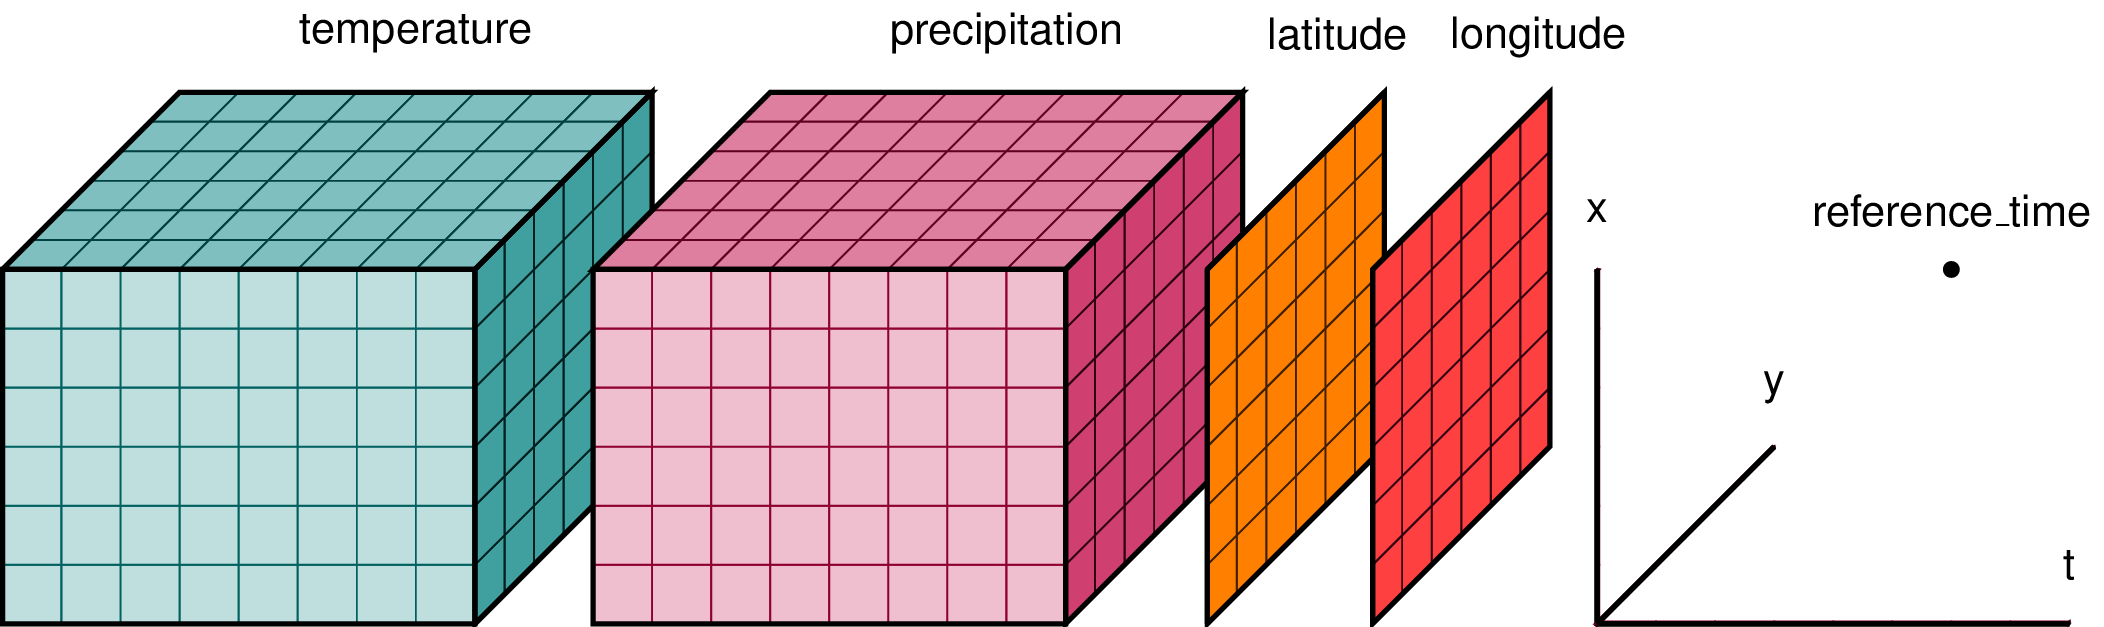
\includegraphics[width=1.00\textwidth]{images/multidimensional-data.png}
\end{frame}

\begin{frame}{Multidimensional Data}
  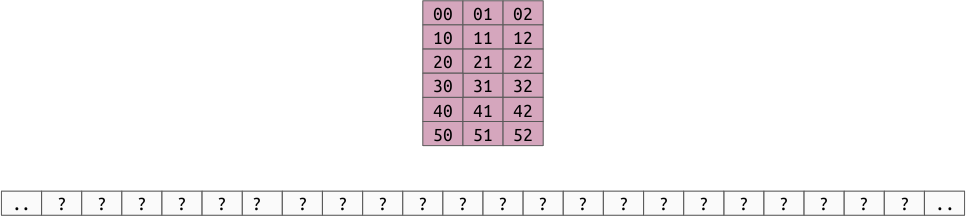
\includegraphics[width=1.00\textwidth]{images/2d-array.png}
\end{frame}

\begin{frame}{Row Order}
  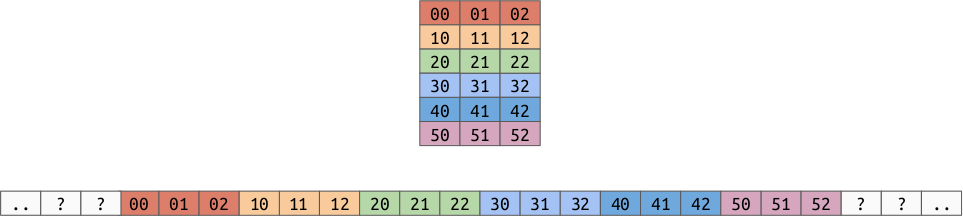
\includegraphics[width=1.00\textwidth]{images/row-order.png}
\end{frame}

\begin{frame}{Column Order}
  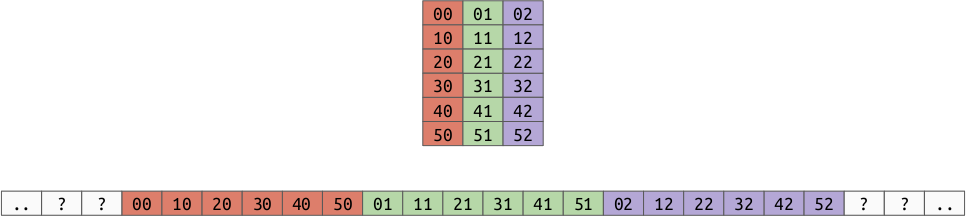
\includegraphics[width=1.00\textwidth]{images/column-order.png}
\end{frame}

\begin{frame}{Chunks}
  \begin{columns}[c]
    \column{0.5\textwidth}
    \begin{center}
      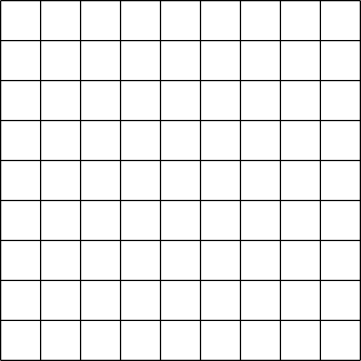
\includegraphics[width=0.8\textwidth]{images/contig-data.png}
    \end{center}

    \column{0.5\textwidth}
    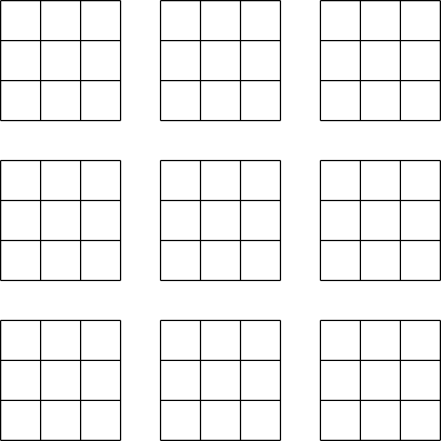
\includegraphics[width=0.8\textwidth]{images/block-chunks.png}
  \end{columns}
\end{frame}

\begin{frame}{Chunks}
  \begin{itemize}
  \item[]<+-> reduce io
  \item[]<+-> facilitate caching
  \item[]<+-> allow extending the shape of the dataset
  \end{itemize}
\end{frame}

\begin{frame}{Hierarchy}
  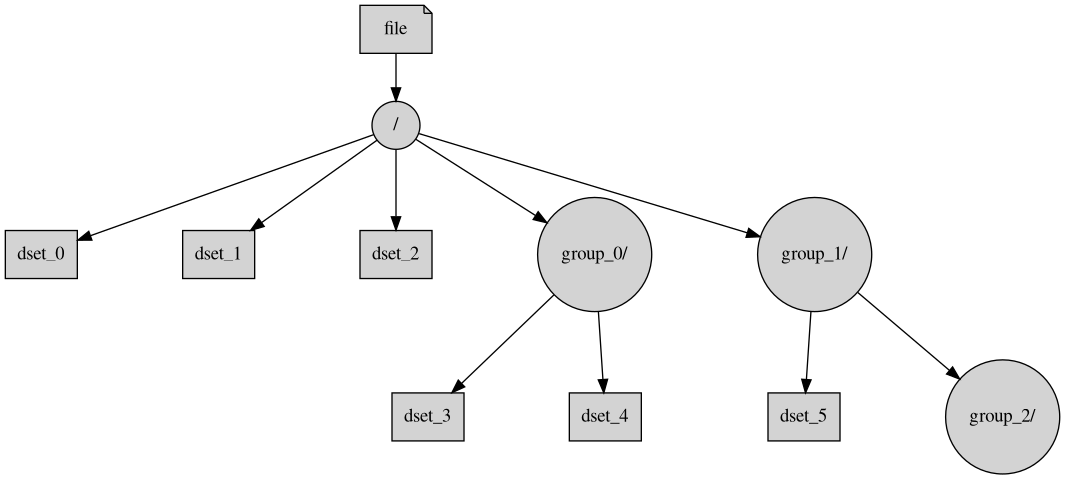
\includegraphics[width=1.0\textwidth]{images/tree.png}
\end{frame}

\begin{frame}{Nodes}
  \begin{definition}[Dataset]
    \begin{itemize}
    \item[] a multidimensional array
    \item[] leaves of a Zarr or HDF5 tree
    \end{itemize}
  \end{definition}
  \pause

  \begin{definition}[Group]
    \begin{itemize}
    \item[] collection of \textbf{datasets} or \textbf{groups}
    \end{itemize}
  \end{definition}
  \pause

  \begin{definition}[Node]
    \begin{itemize}
    \item[] either a \textbf{dataset} or \textbf{group}
    \end{itemize}
  \end{definition}
\end{frame}

\begin{frame}{Attributes}
  \begin{definition}[Attributes]
    \begin{itemize}
    \item[]<+-> key-value data
    \item[]<+-> property of each \textbf{node}
    \end{itemize}
  \end{definition}
\end{frame}

\section{Python Interface}

\begin{frame}{General}
  \begin{itemize}
  \item[]<+-> nested dictionaries
  \item[]<+-> leaves are \textit{array-like}
  \item[]<+-> supports numpy-style indexing
  \item[]<+-> NOTE: describes \hfpy, not \texttt{pytables}
  \end{itemize}
\end{frame}

\begin{frame}[fragile]{\zarr}
  \begin{minted}{python}
>>> import zarr
>>> f = zarr.open('file.zarr')
>>> f
<zarr.hierarchy.Group '/'>
  \end{minted}
  \pause

  \begin{minted}{python}
>>> f['dset'] = np.arange(20 * 5).reshape(20, 5)
>>> f['dset']
>>> <zarr.core.Array '/dset' (20, 5) int64>
\end{minted}
  \pause

  \begin{minted}{python}
>>> f['dset'][10, 3]
53
>>> f['dset'][:]
array([...]])
  \end{minted}
\end{frame}

\begin{frame}[fragile]{\hfpy}
  \begin{minted}{python}
>>> import h5py
>>> f = h5py.File('file.h5')
>>> f
<HDF5 file "file.h5" (mode r+)>
  \end{minted}
  \pause

  \begin{minted}{python}
>>> f['dset'] = np.arange(20 * 5).reshape(20, 5)
>>> f['dset']
<HDF5 dataset "dset": shape (20, 5), type "<i8">
\end{minted}
  \pause

  \begin{minted}{python}
>>> f['dset'][10, 3]
53
>>> f['dset'][:]
array([...]])
  \end{minted}
\end{frame}

\begin{frame}{Extra Functionality}
  \begin{itemize}
  \item[]<+-> \texttt{Node.attrs} to get access to attributes as dict-like object
  \item[]<+-> \texttt{Group.create\_dataset} to set chunk shape and compression
  \item[]<+-> \texttt{Group.create\_group} to create sub-groups
  \item[]<+-> \texttt{Dataset.read\_direct} to read into existing buffers
  \end{itemize}
\end{frame}

\section{Making a Decision}

\begin{frame}{HDF5}
  \begin{itemize}
  \item<+-> over 20 years old
  \item<+-> excellent cross language support
  \item<+-> lots of existing software
  \item<+-> written in (very clean) C
  \item<+-> can be made thread safe, not thread optimal
  \item<+-> extensible in C
  \end{itemize}
\end{frame}

\begin{frame}{Zarr}
  \begin{itemize}
  \item<+-> first release in 2015, 1.0 on May 17 2016
  \item<+-> written in Python, Python oriented
  \item<+-> has specification which could be reimplemented
  \item<+-> multithreading support
  \item<+-> extensible in Python
  \end{itemize}
\end{frame}

\begin{frame}{Extensions}
  \begin{itemize}
  \item[]<+-> filters and compressors
  \item[]<+-> storage backends
  \item[]<+-> which extensions come as part of the library itself?
  \item[]<+-> how to extend the libraries for non-standard use cases?
  \item[]<+-> ease of distributing extensions
  \end{itemize}
\end{frame}

\section{Filters}

\begin{frame}{Filters}
  \begin{definition}[Filter]
    \begin{itemize}
    \item[]<+-> a function that sits between the raw data and the storage
    \item[]<+-> converts data on read and write
    \item[]<+-> act on one chunk at a time
    \item[]<+-> composable
    \item[]<+-> compressors
    \item[]<+-> checksumming
    \end{itemize}
  \end{definition}
\end{frame}
      
\begin{frame}{Filters}
  \begin{columns}
    \column{0.5\textwidth}
    \begin{block}{write}
      \begin{center}
        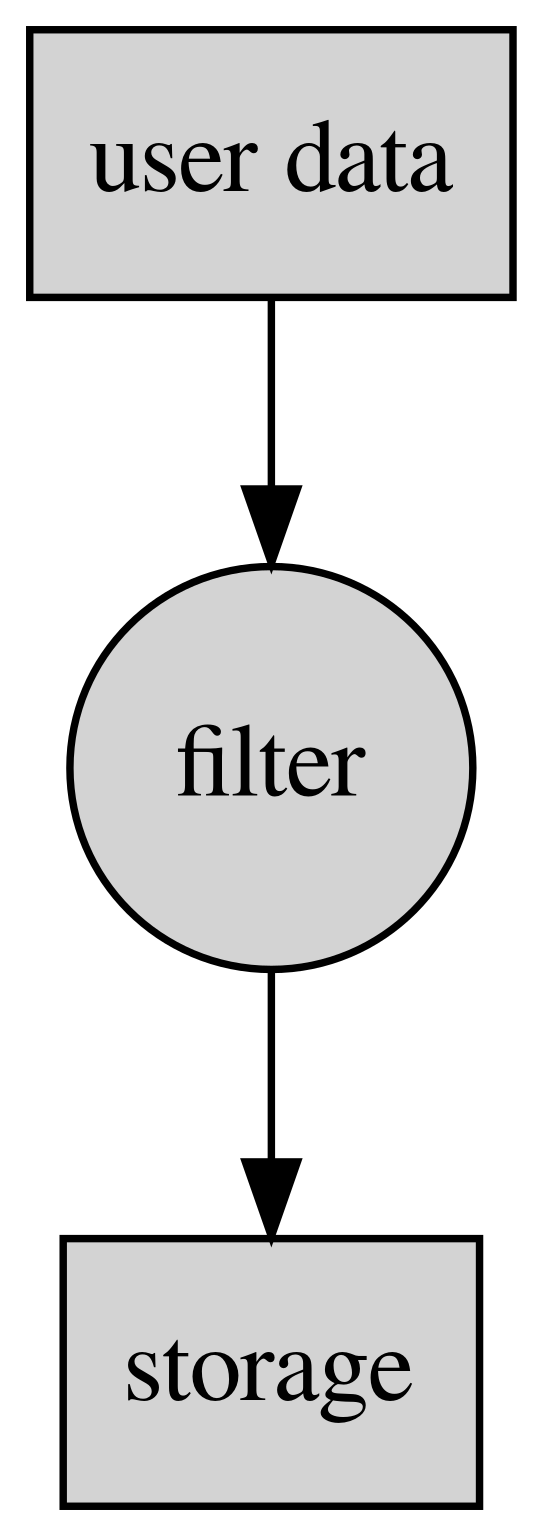
\includegraphics[height=0.75\textheight]{images/write-filter.png}
      \end{center}
    \end{block}

    \column{0.5\textwidth}
    \begin{block}{read}
      \begin{center}
        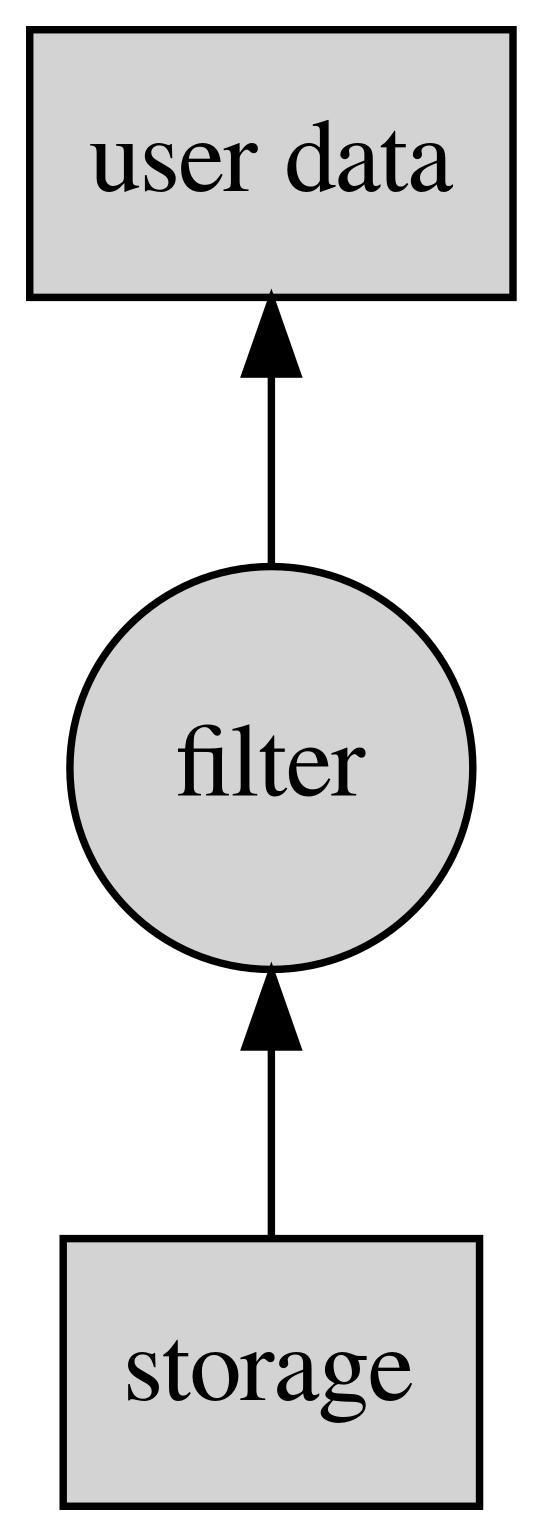
\includegraphics[height=0.75\textheight]{images/read-filter.png}
      \end{center}
    \end{block}
  \end{columns}
\end{frame}

\begin{frame}{Filter Pipelines}
  \begin{columns}
    \column{0.5\textwidth}
    \begin{block}{write}
      \begin{center}
        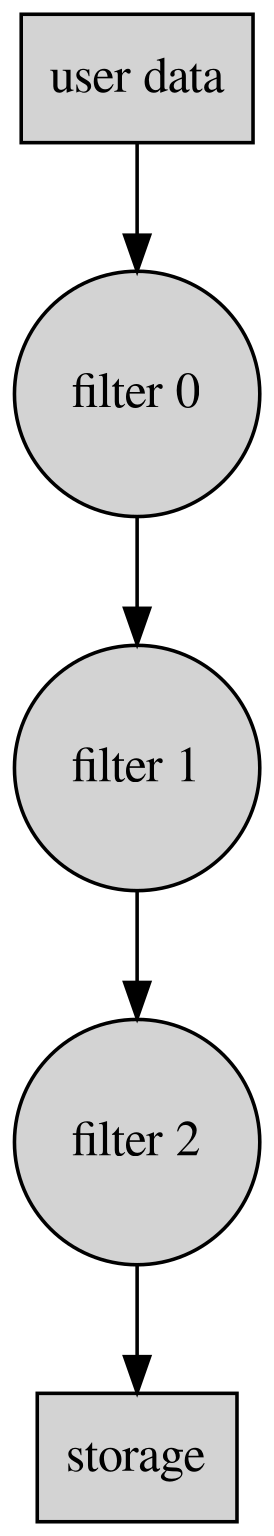
\includegraphics[height=0.75\textheight]{images/write-filter-pipeline.png}
      \end{center}
    \end{block}

    \column{0.5\textwidth}
    \begin{block}{read}
      \begin{center}
        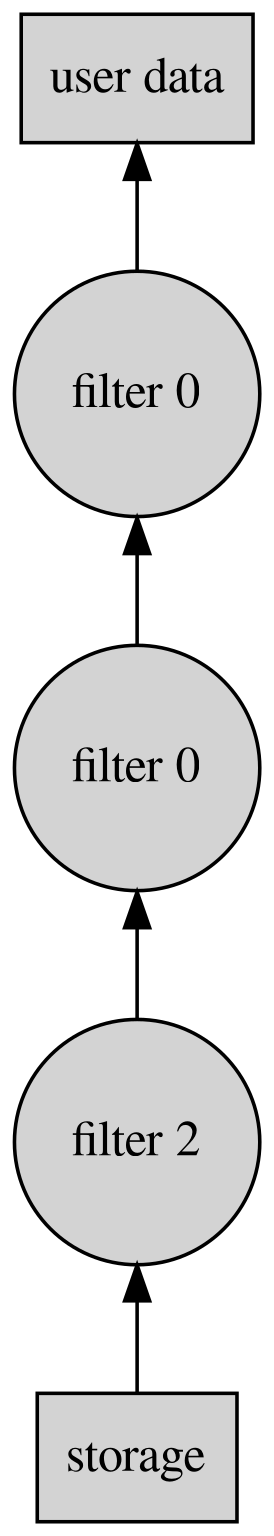
\includegraphics[height=0.75\textheight]{images/read-filter-pipeline.png}
      \end{center}
    \end{block}
  \end{columns}
\end{frame}

\begin{frame}[fragile]{Writing an HDF5 Filter}
  \begin{minted}{c}
size_t dod_filter(unsigned int flags,
                  size_t cd_nelmts,
                  const unsigned int cd_values[],
                  size_t nbytes,
                  size_t *buf_size,
                  void **buf);
  \end{minted}
\end{frame}

\end{document}